\documentclass[11pt]{article}
\usepackage[a4paper, margin=2cm]{geometry}
\usepackage{amsmath}
\usepackage{amssymb}
\usepackage{amsthm}
\usepackage{dsfont}
\usepackage{bbm}
\usepackage{multirow}
\usepackage{array}
\usepackage{diagbox}
\usepackage{makecell}
\newcolumntype{C}[1]{>{\centering\arraybackslash}m{#1}}
% \usepackage{charter}
\usepackage{fontspec}
% \usepackage{unicode-math}
\setmainfont{Charter}
% \setmathfont{XCharter-Math.otf}
% \usepackage{newtxtext,newtxmath}
\usepackage{braket}
\usepackage{slashed}
\usepackage{color}
\usepackage[table]{xcolor}
\usepackage[mathscr]{euscript}
\usepackage{graphicx}
\usepackage{placeins}
\usepackage{floatrow}
\floatsetup[table]{capposition=top}
\usepackage[caption=false]{subfig}
\usepackage[export]{adjustbox}
\floatsetup[figure]{style=plain,subcapbesideposition=top}
\usepackage{xfrac}
\usepackage{bm}
\usepackage{microtype}
\usepackage{commath}
\usepackage{mathtools}
\usepackage{enumitem}
\usepackage{xparse}
\usepackage[
    colorlinks=true, urlcolor=blue,
    linkcolor=blue, citecolor=blue
]{hyperref}% add hypertext capabilities
\usepackage{tikz}
\usepackage{ifthen}
\usepackage[framemethod=TikZ]{mdframed}
\usepackage[version=4]{mhchem}
\usepackage[numbers]{natbib}
\usepackage[nottoc]{tocbibind}
\usepackage[english]{babel}
\usepackage[autostyle, english = american]{csquotes}
\MakeOuterQuote{"}
\usepackage{setspace}

\usetikzlibrary{decorations.markings}
\usetikzlibrary{calc, positioning, arrows.meta}
\tikzset{midarrow/.style={
    decoration={markings, mark=at position 0.55 with {\arrow{>}}},
    postaction={decorate}
}}
\tikzset{midarrowrev/.style={
    decoration={markings, mark=at position 0.45 with {\arrow{<}}},
    postaction={decorate}
}}

% \allowdisplaybreaks

\theoremstyle{remark}
\newtheorem*{remark}{Remark}

\NewDocumentEnvironment{diagram}{O{0.68} O{0.75}}{
    \begin{tikzpicture}[
        baseline = (X.base),
        every node/.style={scale=#1}, scale=#2
    ]
}{\end{tikzpicture}}

\definecolor{green}{RGB}{50, 180, 50}
\definecolor{blue}{RGB}{20, 30, 250}

\newcommand{\pos}[2]{\begin{matrix}
    #1 \\ #2
\end{matrix}}
\newcommand{\dobase}[2]{
    \draw (#1,#2) node (X) {$\phantom{X}$};
}

\NewDocumentCommand{\lineH}{O{black} m m m}{
    \draw[color=#1] (#2,#4) -- (#3,#4);
}
\NewDocumentCommand{\lineHa}{O{black} m m m}{
    \draw[midarrow, color=#1] (#2,#4) -- (#3,#4);
}

\NewDocumentCommand{\lineV}{O{black} m m m}{
    \draw[color=#1] (#4,#2) -- (#4,#3);
}
\NewDocumentCommand{\lineVa}{O{black} m m m}{
    \draw[midarrow, color=#1] (#4,#2) -- (#4,#3);
}

\newcommand{\contrL}[3]{
    \draw (#3,#1) to[out=180,in=180] (#3,#2);
}
\newcommand{\contrLa}[3]{
    \draw[midarrow] (#3,#1) to[out=180,in=180] (#3,#2);
}

\newcommand{\contrR}[3]{
    \draw (#3,#1) to[out=0,in=0] (#3,#2);
}
\newcommand{\contrRa}[3]{
    \draw[midarrow] (#3,#1) to[out=0,in=0] (#3,#2);
}

\NewDocumentCommand{\rect}{m m m m m o}{
    \IfNoValueTF{#6}{
        \draw[rounded corners] 
        (#1 - #3/2, #2 - #4/2) 
        rectangle (#1 + #3/2, #2 + #4/2);
    }{
        \draw[rounded corners, fill=#6] 
        (#1 - #3/2, #2 - #4/2) 
        rectangle (#1 + #3/2, #2 + #4/2);
    }
    \node[align=center] at (#1,#2) {#5};
}

\newcommand{\tensor}[3]{
    \rect{#1}{#2}{1}{1}{#3}
}
\newcommand{\Tensora}[1]{
    \begin{diagram}
        \dobase{0}{0} \tensor{0}{0}{#1}
        \lineHa{-1}{-0.5}{0}
        \lineHa{0.5}{1}{0}
        \lineVa{-1}{-0.5}{0}
    \end{diagram}
}
\newcommand{\TensorAC}[1]{
    \begin{diagram}
        \dobase{0}{0} \tensor{0}{0}{#1}
        \lineHa{-1}{-0.5}{0}
        \lineHa{1}{0.5}{0}
        \lineVa{-1}{-0.5}{0}
    \end{diagram}
}

\newcommand{\tensorL}[3]{
    \draw (-0.5+#1,-0.5+#2) -- (0.25+#1,-0.5+#2) 
    -- (0.5+#1,0+#2) -- (0.25+#1,0.5+#2) 
    -- (-0.5+#1,0.5+#2) -- cycle;
    \draw (#1-0.07,#2) node {#3};
}
\newcommand{\TensorLa}[1]{
    \begin{diagram}
        \dobase{0}{0} \tensorL{0}{0}{#1}
        \lineHa{-1}{-0.5}{0}
        \lineHa{0.5}{1}{0}
        \lineVa{-1}{-0.5}{0}
    \end{diagram}
}

\newcommand{\tensorR}[3]{
    \draw (0.5+#1,-0.5+#2) -- (-0.25+#1,-0.5+#2) 
    -- (-0.5+#1,0+#2) -- (-0.25+#1,0.5+#2) 
    -- (0.5+#1,0.5+#2) -- cycle;
    \draw (#1+0.05,#2) node {#3};
}
\newcommand{\TensorRa}[1]{
    \begin{diagram}
        \dobase{0}{0} \tensorR{0}{0}{#1}
        \lineHa{-1}{-0.5}{0}
        \lineHa{0.5}{1}{0}
        \lineVa{-1}{-0.5}{0}
    \end{diagram}
}

\newcommand{\tensorU}[3]{
    \draw (-0.5+#1,0.5+#2) -- (0.5+#1,0.5+#2) 
    -- (0.5+#1,-0.25+#2) -- (0+#1,-0.5+#2) 
    -- (-0.5+#1,-0.25+#2) -- cycle;
    \draw (#1,#2+0.07) node {#3};
}
\newcommand{\tensorD}[3]{
    \draw (-0.5+#1,-0.5+#2) -- (0.5+#1,-0.5+#2) 
    -- (0.5+#1,0.25+#2) -- (0+#1,0.5+#2) 
    -- (-0.5+#1,0.25+#2) -- cycle;
    \draw (#1,#2-0.05) node {#3};
}

\newcommand{\fuserL}[5]{
    \draw (#1,#2-#3) -- (#1,#2+#3) 
    -- (#1-#4,#2) -- cycle;
    \node at (#1-0.4*#4,#2) {#5};
}
\newcommand{\fuserR}[5]{
    \draw (#1,#2-#3) -- (#1,#2+#3) 
    -- (#1+#4,#2) -- cycle;
    \node at (#1+0.4*#4,#2) {#5};
}

\NewDocumentCommand{\mat}{O{0.5} m m m}{
    \draw (#2,#3) circle (#1);
    \draw (#2,#3) node {#4};
}
\NewDocumentCommand{\Matrixa}{O{0.5} m}{
    \begin{diagram}
        \dobase{0}{0} \mat[#1]{0}{0}{#2}
        \lineHa{#1}{1}{0} \lineHa{-1}{-#1}{0}
    \end{diagram}
}
\NewDocumentCommand{\MatrixC}{O{0.5} m}{
    \begin{diagram}
        \dobase{0}{0} \mat[#1]{0}{0}{#2}
        \lineHa{1}{#1}{0} \lineHa{-1}{-#1}{0}
    \end{diagram}
}

\NewDocumentCommand{\weight}{O{0.5} m m m}
{\begin{scope}[shift={(#2,#3)}]
    \draw (-#1,0) -- (0,#1) -- (#1,0) -- (0,-#1) -- cycle;
    \node at (0,0) {#4};
\end{scope}}

\NewDocumentCommand{\bloba}{m m m m m}{
    % Get the parameters
    \def\xc{#1}
    \def\yc{#2}
    \def\inangles{#3}
    \def\outangles{#4}
    % Draw the circle at the specified coordinates
    \draw (\xc,\yc) circle (0.5);
    % Draw incoming arrows
    \foreach \angle in \inangles {
        \pgfmathsetmacro{\xstart}{\xc + 1.5*cos(\angle)}
        \pgfmathsetmacro{\ystart}{\yc + 1.5*sin(\angle)}
        \pgfmathsetmacro{\xend}{\xc + 0.5*cos(\angle)}
        \pgfmathsetmacro{\yend}{\yc + 0.5*sin(\angle)}
        \draw[midarrow] (\xstart, \ystart) -- (\xend, \yend);
    }
    % Draw outgoing arrows
    \foreach \angle in \outangles {
        \pgfmathsetmacro{\xstart}{\xc + 0.5*cos(\angle)}
        \pgfmathsetmacro{\ystart}{\yc + 0.5*sin(\angle)}
        \pgfmathsetmacro{\xend}{\xc + 1.5*cos(\angle)}
        \pgfmathsetmacro{\yend}{\yc + 1.5*sin(\angle)}
        \draw[midarrow] (\xstart, \ystart) -- (\xend, \yend);
    }
    \draw (#1,#2) node {#5};
}

\NewDocumentCommand{\blob}{m m m m}{
    % Get the parameters
    \def\xc{#1}
    \def\yc{#2}
    \def\angles{#3}
    % Draw the circle at the specified coordinates
    \draw (\xc,\yc) circle (0.5);
    % Draw incoming arrows
    \foreach \angle in \angles {
        \pgfmathsetmacro{\xstart}{\xc + 1.5*cos(\angle)}
        \pgfmathsetmacro{\ystart}{\yc + 1.5*sin(\angle)}
        \pgfmathsetmacro{\xend}{\xc + 0.5*cos(\angle)}
        \pgfmathsetmacro{\yend}{\yc + 0.5*sin(\angle)}
        \draw (\xstart, \ystart) -- (\xend, \yend);
    }
    \draw (#1,#2) node {#4};
}

\newcommand{\closeLeft}[2]
{\begin{scope}[shift={(#1,0)}]
    \draw (-1,0.5) to[out=90,in=180] (0,1.5);
    \draw (0,-1.5) to[out=180,in=270] (-1,-0.5);
    \mat{-1}{0}{#2}
\end{scope}}
\newcommand{\closeLefta}[2]
{\begin{scope}[shift={(#1,0)}]
    \draw[midarrow] (-1,0.5) to[out=90,in=180] (0,1.5);
    \draw[midarrow] (0,-1.5) to[out=180,in=270] (-1,-0.5);
    \mat{-1}{0}{#2}
\end{scope}}

\newcommand{\closeRight}[2]{
    \draw (#1,+1.5) to[out=0,in=90] (#1+1,0.5);
    \draw (#1+1,-0.5) to[out=270,in=0] (#1,-1.5);
    \mat{#1+1}{0}{#2}
}
\newcommand{\closeRighta}[2]{
    \draw[midarrow] (#1+1,0.5) to[out=90,in=0] (#1,+1.5);
    \draw[midarrow] (#1,-1.5) to[out=0,in=-90] (#1+1,-0.5);
    \mat{#1+1}{0}{#2}
}

\newcommand{\colmat}[3]{
    \tensor{#1}{1.5}{#2}
    \tensor{#1}{-1.5}{#3}
    \lineV{-1}{1}{#1}
}
\newcommand{\colmata}[3]{
    \tensor{#1}{1.5}{#2}
    \tensor{#1}{-1.5}{#3}
    \lineVa{-1}{1}{#1}
}

\newcommand{\colmatL}[3]{
    \tensorL{#1}{1.5}{#2}
    \tensorL{#1}{-1.5}{#3}
    \lineV{-1}{1}{#1}
}
\newcommand{\colmatLa}[3]{
    \tensorL{#1}{1.5}{#2}
    \tensorL{#1}{-1.5}{#3}
    \lineVa{-1}{1}{#1}
}

\newcommand{\colmatR}[3]{
    \tensorR{#1}{1.5}{#2}
    \tensorR{#1}{-1.5}{#3}
    \lineV{-1}{1}{#1}
}
\newcommand{\colmatRa}[3]{
    \tensorR{#1}{1.5}{#2}
    \tensorR{#1}{-1.5}{#3}
    \lineVa{-1}{1}{#1}
}

\newcommand{\applyTransferL}[3]{
    \begin{diagram}
        \dobase{0}{0}
        \colmat{0}{#1}{#3} \closeLeft{-0.5}{#2}
        \lineH{0.5}{1}{1.5} \lineH{0.5}{1}{-1.5}
    \end{diagram}
}
\newcommand{\applyTransferLa}[3]{
    \begin{diagram}
        \dobase{0}{0}
        \colmata{0}{#1}{#3} 
        \closeLefta{-0.5}{#2}
        \lineHa{0.5}{1}{1.5} 
        \lineHa{1}{0.5}{-1.5}
    \end{diagram}
}

\newcommand{\applyTransferR}[3]{
    \begin{diagram}
        \dobase{0}{0}
        \colmat{0}{#1}{#3} \closeRight{0.5}{#2}
        \lineH{-0.5}{-1}{1.5} \lineH{-0.5}{-1}{-1.5}
    \end{diagram}
}

\newcommand{\lrtimesMPS}[3]{
    \begin{diagram}
        \dobase{0}{0}
        \lineH{-3}{-2.5}{0}
        \mat{-2}{0}{#1}
        \lineH{-1.5}{-0.5}{0}
        \tensor{0}{0}{#2}
        \lineV{-1}{-0.5}{0}
        \lineH{0.5}{1.5}{0}
        \mat{2}{0}{#3}
        \lineH{2.5}{3}{0}
    \end{diagram}
}
\newcommand{\lrtimesMPSa}[3]{
    \begin{diagram}
        \dobase{0}{0}
        \lineHa{-3}{-2.5}{0}
        \mat{-2}{0}{#1}
        \lineHa{-1.5}{-0.5}{0}
        \tensor{0}{0}{#2}
        \lineVa{-1}{-0.5}{0}
        \lineHa{0.5}{1.5}{0}
        \mat{2}{0}{#3}
        \lineHa{2.5}{3}{0}
    \end{diagram}
}

\newcommand{\ltimesMPS}[2]{
    \begin{diagram}
        \dobase{0}{0}
        \mat{0}{0}{#1}
        \tensor{2}{0}{#2}
        \lineH{-1}{-0.5}{0}
        \lineH{0.5}{1.5}{0}
        \lineH{2.5}{3}{0}
        \lineV{-1}{-0.5}{2}
    \end{diagram}
}
\newcommand{\ltimesMPSa}[2]{
    \begin{diagram}
        \dobase{0}{0}
        \mat{0}{0}{#1}
        \tensor{2}{0}{#2}
        \lineHa{-1}{-0.5}{0}
        \lineHa{0.5}{1.5}{0}
        \lineHa{2.5}{3}{0}
        \lineVa{-1}{-0.5}{2}
    \end{diagram}
}

\newcommand{\rtimesMPS}[2]{
    \begin{diagram}
        \dobase{0}{0}
        \tensor{0}{0}{#1}
        \mat{2}{0}{#2}
        \lineH{-1}{-0.5}{0}
        \lineH{0.5}{1.5}{0}
        \lineH{2.5}{3}{0}
        \lineV{-1}{-0.5}{0}
    \end{diagram}
}
\newcommand{\rtimesMPSa}[2]{
    \begin{diagram}
        \dobase{0}{0}
        \tensor{0}{0}{#1}
        \mat{2}{0}{#2}
        \lineHa{-1}{-0.5}{0}
        \lineHa{0.5}{1.5}{0}
        \lineHa{2.5}{3}{0}
        \lineVa{-1}{-0.5}{0}
    \end{diagram}
}

% --------------------------------
% Special math fonts and notations
% --------------------------------

\newcommand{\graphics}[2]{\includegraphics[totalheight={#1}]{#2}}
\newcommand{\tr}{\operatorname{tr}}
\newcommand{\Abs}[1]{
    \left\lVert #1 \right\rVert
}
\newcommand{\bs}[1]{\boldsymbol{#1}}
\newcommand{\p}{\mathsf{P}}
\newcommand{\h}[1]{\ensuremath{\hat{#1}}}
\renewcommand{\t}[1]{\ensuremath{\tilde{#1}}}
\newcommand{\Z}{\ensuremath{\mathbb{Z}}}
\newcommand{\C}{\ensuremath{\mathbb{C}}}
\newcommand{\R}{\ensuremath{\mathbb{R}}}
\newcommand{\voperator}[1]{\ensuremath{\breve{#1}}}
\newcommand{\manifold}[1]{\ensuremath{\mathcal{#1}}}
\newcommand{\group}[1]{\ensuremath{\mathsf{#1}}}
\newcommand{\vectorspace}[1]{\ensuremath{\mathbb{#1}}}
\newcommand{\algebra}[1]{\ensuremath{\mathfrak{#1}}}
\newcommand{\pf}{\operatorname{pf}}

\newcommand{\Imag}{\mathrm{Im}}
\newcommand{\Real}{\mathrm{Re}}
\newcommand{\sgn}{\mathrm{sgn}}
\newcommand{\T}{\mathsf{T}}
\newcommand{\diag}{\mathrm{diag}}

\newcommand{\e}{\ensuremath{\mathrm{e}}}
\renewcommand{\d}{\ensuremath{\mathrm{d}}}
\renewcommand{\dag}{^\dagger}
\newcommand{\one}{\mathds{1}}
\newcommand{\ol}[1]{\overline{#1}}

\newcommand{\bA}{\bar{A}}
\newcommand{\tA}{\tilde{A}}
\newcommand{\bB}{\bar{B}}
\newcommand{\bG}{\bar{G}}
\newcommand{\tC}{\tilde{C}}

\newcommand{\vect}[1]{\ensuremath{\boldsymbol{#1}}}
\newcommand{\lv}{\ensuremath{\vect{v}_L^\dagger}}
\newcommand{\rv}{\ensuremath{\vect{v}_R}}
\newcommand{\spst}{\ensuremath{\ket{\{s\}}}}
\newcommand{\E}[2]{\ensuremath{E^{#1}_{#2}}}
\renewcommand{\O}[2]{\ensuremath{O^{#1}_{#2}}}
\renewcommand{\H}[4]{\ensuremath{H^{#1#2}_{#3#4}}}
\newcommand{\I}[6]{\ensuremath{I^{#1#2#3}_{#4#5#6}}}
\newcommand{\HH}[6]{\ensuremath{H^{#1#2#3}_{#4#5#6}}}
\newcommand{\J}[4]{\ensuremath{J^{#1#2}_{#3#4}}}
\newcommand{\alphap}{\ensuremath{{\alpha'}}}
\newcommand{\betap}{\ensuremath{{\beta'}}}
\newcommand{\gammap}{\ensuremath{{\gamma'}}}

% group theory
\newcommand{\U}{\ensuremath{\mathrm{U}}}
\newcommand{\SU}{\ensuremath{\mathrm{SU}}}
\newcommand{\su}{\ensuremath{\mathfrak{su}}}
\newcommand{\SO}{\ensuremath{\mathrm{SO}}}
\newcommand{\so}{\ensuremath{\mathfrak{so}}}

% category theory
\newcommand{\Hom}{\ensuremath{\mathrm{Hom}}}

\graphicspath{{./images/}}

\begin{document}

\section{Tensor network renormalization}\label{sec:tnr-review}

In this section we review the loop-TNR algorithm for tensor networks with periodic boundary condition on a bipartite square lattice (see Fig.~\ref{fig:tnr}a) \cite{Yang2017}. 
The generalization to fermionic tensors is straightforward, which amounts to adding arrows on all bonds and insert $P$ tensors at proper places in the tensor diagrams. 
Suppose that the number of \(T_A\) in the network is \(N\), then the tensor network is denoted as \(\tr(T_A^N T_B^N)\). A complete round of TNR consists of the following steps.

\begin{figure}[h]
    \centering
    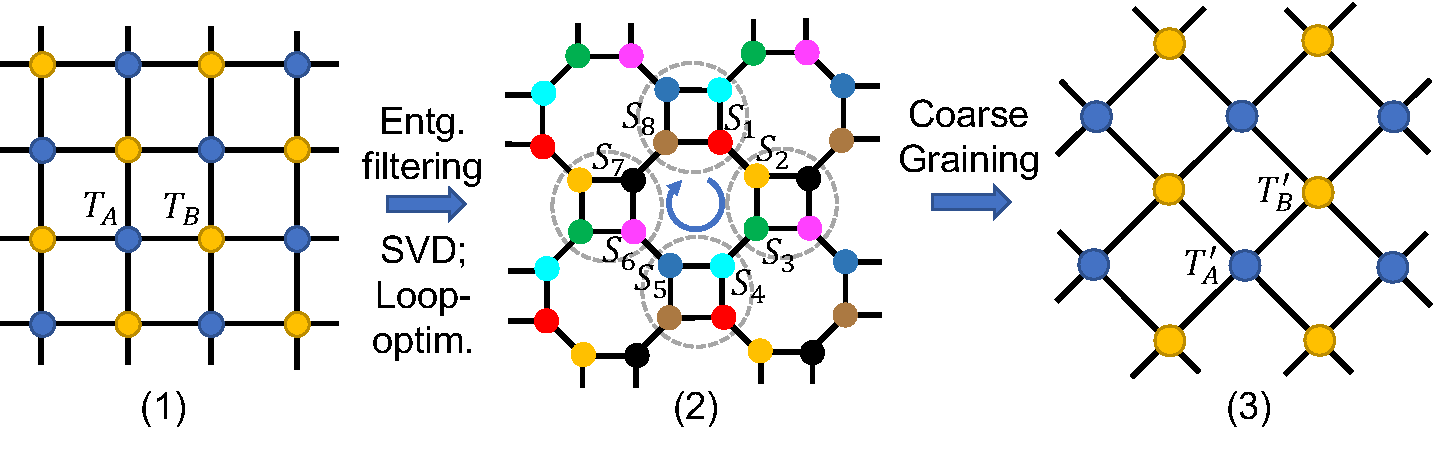
\includegraphics[scale=0.5]{coarsegrain.pdf}
    \caption{A complete round of TNR. (a) A square lattice tensor network containing two types of tensors \(T_A, T_B\). (b) Mixed octagon-square tensor network after SVD of \(T_A, T_B\) and loop optimization. (c) The coarse-grained tensor network after recombining the \(S\) tensors to new \(T'_A, T'_B\). }
    \label{fig:tnr}
\end{figure}

\begin{itemize}
    \item \emph{Entanglement filtering}: To remove short-range entanglement, including the CDL structure in the tensor network, an entanglement filtering step is first performed. Regarding a square in the network as an MPS with periodic boundary condition, standard MPS canonicalization algorithms is applied to find projectors on the links of the network. Then the projectors are absorbed into the network tensors, removing the CDL structure. 
    
    \item \emph{Tensor decomposition}: We perform singular value decomposition (SVD) of \(T_A, T_B\)
    \begin{equation}
    \arraycolsep=1em
    \begin{matrix}
        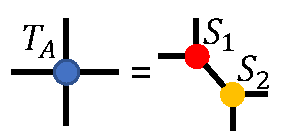
\includegraphics[scale=0.65]{svd_TA.pdf}
        &
        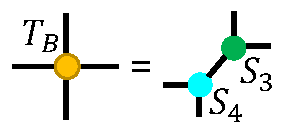
\includegraphics[scale=0.65]{svd_TB.pdf}
    \end{matrix}
    \end{equation}
    Here each \(S\) tensor absorbs the square root of the diagonal singular value matrix, and only the largest \(\chi\) singular values are kept to keep the axis dimension of the resulting tensor small. Then we obtain a mixture of octagons and squares of \(S\) tensors.

    \item \emph{Loop optimization}: The loop-optimization step, which is the most important improvement compared to TRG, reduces the error due to the SVD truncation by minimizing the cost function
    \begin{equation}
        f(S_1, ..., S_8)
        = \left| \begin{matrix}
            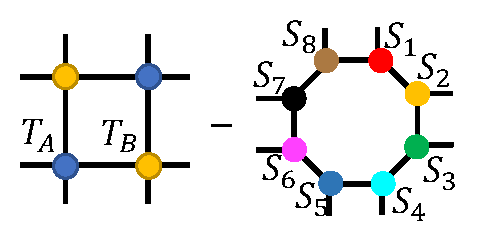
\includegraphics[scale=0.6]{loop_cost.pdf}
        \end{matrix} \right|^2
    \end{equation}
    with respect to the eight rank-3 tensors $S_1, ..., S_8$, where \(| \cdot |\) means the Frobenius 2-norm. Before the optimization \((S_1,S_2) = (S_6,S_5)\) and \((S_3,S_4) = (S_8,S_7)\), but afterwards they are in general different. The minimization is done iteratively with respect to each \(S_i\) while keeping other \(S\) tensors fixed, which amounts to solving a set of linear equations. In practice it is hard to reach convergence in this step, so one usually set a maximum number of "sweeps" over the \(S\) tensors (usually between 100 and 200) after which the program quits the optimization process.

    \item \emph{Coarse-graining}: The eight \(S\) tensors from the loop optimization step is recombined to new \(T'_A, T'_B\) tensors:
    \begin{gather}
        T'_A = \begin{matrix}
            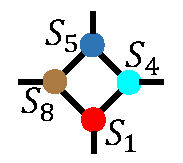
\includegraphics[scale=0.65]{TA-merge.pdf}
        \end{matrix}
        , \quad
        T'_B = \begin{matrix}
            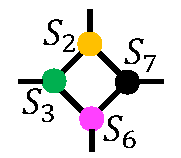
\includegraphics[scale=0.65]{TB-merge.pdf}
        \end{matrix}
    \end{gather}
    The dimension of each axis of \(T'_A, T'_B\) is \(\chi\). Then we normalize the tensors as
    \begin{equation}
        \mathcal{T}'_A = T'_A/f, \quad
        \mathcal{T}'_B = T'_B/f
    \end{equation}
    with the factor \(f > 0\) commonly chosen as
    \begin{equation}
        f = |\tr[(T'_A T'_B)^2]|^{1/4}
        = \left|\ \ \begin{matrix}
            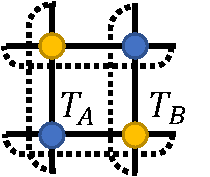
\includegraphics[scale=0.6]{norm_ab.pdf}
        \end{matrix}
        \right|^{1/4}
    \end{equation}
    Now the number of tensors in the network is reduced by a half. The normalized \(\mathcal{T}'_A, \mathcal{T}'_B\) serve as the input of the next round of TNR. We note that the TNR algorithm can also be applied to networks of other lattice types (such as the triangular and the honeycomb lattices) with minor modifications of the coarse-graining step.
\end{itemize}

\subsection{Fixed point tensor and conformal data}

The TNR algorithm can help us identify the conformal field theory (CFT) that describes the critical point of phase transition. After several steps of coarse-graining, the tensor gradually flows to the fixed point corresponding to a CFT. One tensor now represents a large patch of the original network. By constructing a \emph{transfer matrix} of $w \times h$ tensors along the space (horizontal) direction 
\begin{equation}
    \begin{matrix}
        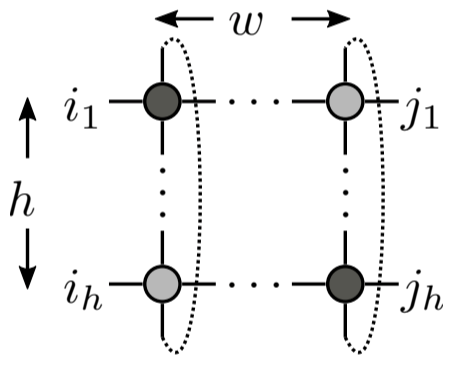
\includegraphics[scale=0.4]{transfer_mat.png}
    \end{matrix}
\end{equation}
the scaling dimensions are related to the eigenvalues (sorted from large to small in magnitude) of the matrix by \cite{gu2009tensor}

\begin{equation}
    \Delta_i = -\frac{1}{2\pi \operatorname{Im}\tau} 
    \ln \left| \frac{\lambda_i}{\lambda_0} \right|, \quad
    \tau = i \frac{w}{vh}
\end{equation}

The additional coefficient $v$ describes the degree of isotropy of the space-time lattice which will be adjusted to 1 (it is always equal to 1 for classical 2D models, and does not need tuning).

\subsection{Benchmark: (1+1)D spinless fermion model}

We benchmark the performance of the fermionic version of loop-TNR with a (1 + 1)D spinless fermion model \cite{BaoThesis2019}
\begin{equation} \label{eq:spinless-fermion}
    H = -t \sum_i 
    (c_i^\dagger c_{i+1} + c_{i+1}^\dagger c_i) 
    + V \sum_i \left(n_i - \frac{1}{2}\right)\left(n_{i+1} - \frac{1}{2}\right)
\end{equation}
where $n_i = c_i^\dagger c_i$, $t,V > 0$ and we usually set $t = 1$. This model can be mapped from the spin-1/2 Heisenberg XXZ chain via Jordan-Wigner transformation \cite{Senechal2004}; the isotropic case corresponds to $V = 2t$. We consider only $-2t \le V \le 2t$, when the spin model is in the Luttinger liquid phase. The  is described by the compactified boson CFT, with scaling dimensions given by the formula \cite{FrancescoCFT} (the descendants are not included)
\begin{equation} \label{eq:boson-cft}
    \Delta_{e,m} = \frac{e^2}{R^2} + \frac{m^2 R^2}{4}
    \quad (e,m \in \mathbb{Z})
\end{equation}
where $R$ is the compactification radius, related to $t, V$ by
\begin{equation} \label{eq:radius}
    R^2 = 2(1 - g), \quad 
    g = \frac{1}{\pi} \arccos \frac{V}{2t}
\end{equation}
In Figure \ref{fig:spinless-fermion} we compare the loop-TNR result and CFT prediction (corresponding to the combination of APBC, even parity and PBC, odd parity \cite{Senechal2004}) and see good match for $0.1 < g < 0.8$. When $g$ is close to either $0$ or $1$, the algorithm is affected by {\color{red} some other physical reasons}.
\begin{figure}[ht]
    \centering
    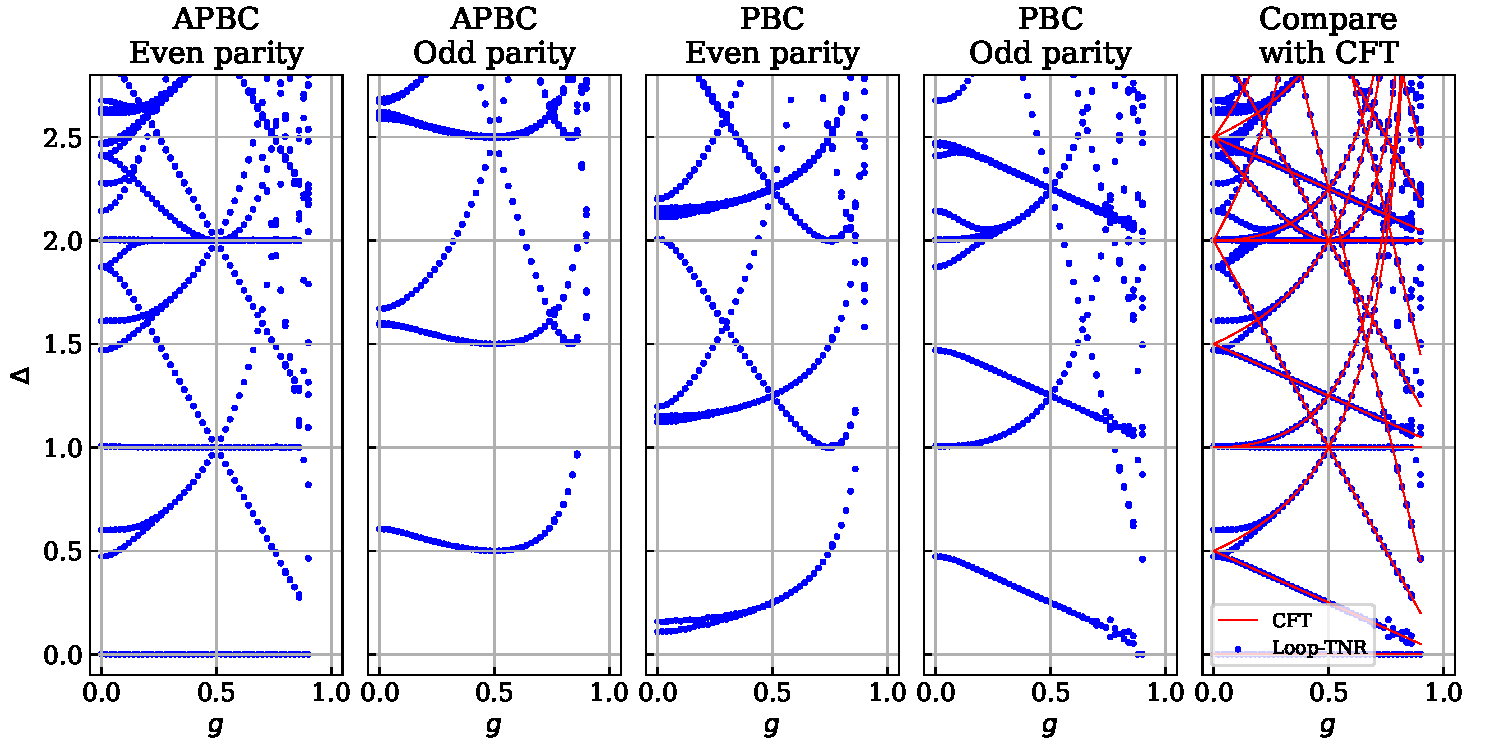
\includegraphics[scale=0.65]{radius.pdf}
    \caption{
        Scaling dimensions extracted from loop-TNR and comparison with CFT prediction Eqs. \eqref{eq:boson-cft} and \eqref{eq:radius} for (1+1)D spinless fermion model Eq. \eqref{eq:spinless-fermion}.
    }
    \label{fig:spinless-fermion}
\end{figure}

\bibliographystyle{ieeetr}
\bibliography{./refs}

\end{document}
